%-------------------------------------------------------------------------------
% rc_file
%-------------------------------------------------------------------------------
%
% \file        rc_file.tex
% \library     Documents
% \author      Chris Ahlstrom
% \date        2015-08-31
% \update      2018-11-11
% \version     $Revision$
% \license     $XPC_GPL_LICENSE$
%
%     Provides the rc_file.
%
%-------------------------------------------------------------------------------

\section{Seq66 "rc" Configuration File}
\label{sec:rc_file}

   There are two \textsl{Seq66} configuration files:
   \texttt{seq66.rc} and \texttt{seq66.usr}.
   See \sectionref{sec:usr_file}; it describes the "usr" file,
   is handled a bit differently than the "rc" file.

   \index{seq66.rc}
   The \textsl{Seq66} configuration file originally was
   named \texttt{.seq24rc},
   and it was stored directly in the user's \texttt{\$HOME} directory,
   following the convention of \textsl{Seq24}.
   To avoid interference with one's existing installation of 
   \textsl{Seq24}, we created a new file
   to take its place, with a fall-back to the original file-name if the new
   file does not exist, or if \textsl{Seq66} is running in
   \index{legacy mode}
   legacy mode.
   In addition, one can change the configuration directory and the base name of
   the "rc" and "usr" files from the command-line.

   After you run \textsl{Seq66} for the first time (in non-legacy
   mode), it will generate a \texttt{seq66.rc} file in your home
   \textsl{configuration} directory:

   \begin{verbatim}
      /home/ahlstrom/.config/seq66/seq66.rc
   \end{verbatim}

   It contains the the data for remote MIDI control, computer keyboard
   control, MIDI clock, JACK transport, and a few other settings.

   \textsl{Seq66} will
   \textsl{always} overwrite the \texttt{sequencer6.rc} file upon
   quitting.  One must therefore quit \textsl{Seq66} before making
   manual modifications to the \texttt{seq66.rc} file.
   Note that many of
   its settings can be modified in the \textbf{Options} dialog
   (see \sectionref{subsubsec:menu_file_options}).
   There is an old, but complete, example of the \textsl{Seq24}
   "rc" file at \cite{seq24launchpadmapper}.
   It includes a setup for the
   Novation Launchpad device.

   Now let's covered each section of the "rc" file in order.

\subsection{"rc" File / Comments}
\label{subsec:rc_file_midi_comments}

   The very top of the "rc" file that \textsl{Seq66} generates is a stock
   banner showing the version of \textsl{Seq66} to which this file
   applies, the name of the configuration file, and when it was written.  The
   user can also add a comments section that explain what the user's setup is
   in brief:

   \begin{verbatim}
   [comments]

   Comments added to this section are preserved.  Lines starting with
   a '#' or '[', or that are blank, are ignored.  Start lines that must
   be blank with a space.
   \end{verbatim}

   A blank line (not even a space) ends the comment section.

\subsection{"rc" File / MIDI Control}
\label{subsec:rc_file_midi_control}

   Like \textsl{Seq24}, \textsl{Seq66} provides a way to control the
   application to some extent via a MIDI controller, such as a MIDI keyboard or
   a MIDI pad device.  The current section describes this feature;
   additional resources and ideas can be found at \url{linuxaudio.org}
   (\cite{midicontrol}).

   \index{[midi-control-file]}
   New with version 0.96 of \textsl{Seq66} is the ability
   to offload the MIDI control section to a separate file.  Simply move
   the whole \texttt{[midi-control]} section to a separate file in
   the \textsl{Seq66} configuration directory, and add the following
   snippet:

   \begin{verbatim}
   [midi-control-file]
      nanomap.rc        # contains a whole [midi-control] section
   \end{verbatim}

   As with the normal "rc", this file is rewritten upon exit, so
   don't bother trying to add comments to it.  The rest of this section
   applied either to that "rc" or the normal "rc" file.

   \index{[midi-control]}
   The MIDI control section begins with the following "INI"-style
   group marker tag:

   \begin{verbatim}
   [midi-control]
      74      # MIDI controls count (74/84/96)
   \end{verbatim}

   The number (74) is the number of lines in the MIDI Control section.  The
   extended automation values bring this number up to 84, and the most recent
   version of \textsl{Seq66} brings this up to 96.  Note that earlier
   version will complain about numbers higher than what they can handle.  If
   so, edit the "rc" file to reduce that number.

   Even in the latest version of \textsl{Seq66}, 
   not all of these new values are yet usable, and there are also some values
   reserved for future expansion.  Currently, the
   "start", "pause", "stop", and "bpm" page controls, and the "performance
   record", "MIDI THRU", "MIDI RECORD", "MIDI Quantized RECORD",
   and play-list control have been implemented.
   Each MIDI control line has the following format:

   \begin{verbatim}
      74     [0 0 0 0 0 0]   [0 0 0 0 0 0]   [0 0 0 0 0 0]
   \end{verbatim}

   The first number is an \textsl{internal} control number ranging from
   0 to 73, 83, or 95 depending on the version of \textsl{Seq66}.
   The three bracketed sections represent MIDI controls to
   \index{[midi-control]!toggle}
   toggle,
   \index{[midi-control]!on}
   turn on, and
   \index{[midi-control]!off}
   turn off a pattern or mute group.
   However, some MIDI controls extend the meanings of these brackets
   for additional functionality.

   \begin{verbatim}
               ------------------ on/off
              | ----------------- inverse
              | |  -------------- MIDI status (event) byte (e.g. note on)
              | | |  ------------ data 1 (e.g. note number)
              | | | |  ---------- data 2 min
              | | | | |  -------- data 2 max
              | | | | | |
              v v v v v v
      74     [0 0 0 0 0 0]   [0 0 0 0 0 0]   [0 0 0 0 0 0]
    Index:    Toggle          On              Off
    Playback: Pause           Start/Play      Stop
    Playlist: By-Value        Next            Previous
   \end{verbatim}

   The first number is an index number, starting at 0.  It indicates what
   function the control line will affect.
   The numbers in the leftmost brackets define a \textsl{toggle} filter;
   the numbers in the middle brackets define a \textsl{on} filter;
   the numbers in the rightmost brackets define a \textsl{off} filter.
   Additional functions are shown that extend these basic functions,
   such as changing a selection, controlling playback, or activating a feature.

   The numbers inside the brackets define six values that set up the control.
   The layout of each filter inside the brackets is as follows:

      \textbf{[OPR INV STAT D1 D2min D2max]}

   \begin{itemize}
      \item \textbf{OPR} = \textbf{on/off}
      \item \textbf{INV} = \textbf{inverse}
      \item \textbf{STAT} = \textbf{MIDI status byte} (channel ignored) 
      \item \textbf{D1} = \textbf{data1}
      \item \textbf{D2min} = \textbf{data2 min}
      \item \textbf{D2max} = \textbf{data2 max}
   \end{itemize}

   If \textbf{OPR (on/off)} is set to 1, it will match the incoming MIDI
   against the \textbf{STAT (MIDI status byte)} pattern.
   and perform the action (on/off/toggle) if the data
   falls in the range specified.  All values are in decimal.

   \textbf{Note}: In legacy versions (\textsl{Seq24} and early versions
   of \textsl{Seq66}), the channel nybble of the MIDI control (and all
   other incoming MIDI events) were stripped off.
   This is no longer the case, and thus opens up many more events useful for
   MIDI control.   But do note that events that are actually recorded end up
   getting the channel number of the pattern into which they are recorded.

   The \textbf{INV (inverse)} field will make the pattern perform the opposite
   action (\textsl{off} for \textsl{on}, \textsl{on} for \textsl{off}) if the
   data falls outside the specified range.  This is cool because one can map
   several sequences to a knob or fader.

   The \textbf{STAT (MIDI status byte)} field is a MIDI status byte number in
   decimal notation.  The channel nybble of this byte is ignored.  One can look
   up the possible status values up in the MIDI messages tables; the relevant
   data can be found at \cite{midicontroltable}.  As the channel on which the
   events are sent is ignored, it is sufficient to use the values for channel
   1; that is, 0.

   The last three fields describe the range of data that will match.  The
   \textbf{D1 (data1)} field provides the actual MIDI event message number to
   detect, in decimal.  This item could be a Note On/Off event or a
   Control/Mode change event, for example.

   The \textbf{D2min (data2 min)} field is the minimum value of the event for
   the filter to match. For Note On/Off events, this would be the velocity
   value, for example.

   The \textbf{D2max (data2 max)} field is the maximum value of the event for
   the filter to match.

%  This set of values is explained below.

   For each pattern, we can set up MIDI events to turn a 
   pattern on, off, or to toggle it, or to control some other function.
   If the incoming MIDI event value matches a value present in the filter, it
   will \textsl{toggle} (first field), \textsl{enable} (second field) or
   \textsl{disable} (third field) the sequence, or perform some kind of automation
   control.

   As a quick example, let us set up a Note On event on channel 2 and key value
   48 that will increment \textsl{Seq66}'s BPM value each time it is
   pressed.  A Note On event is 0x90 hex, or 144 decimal.  Channel 2 is 0x1 hex
   or 1 decimal.   Adding the Note On value to the the channel number yields
   0x91 hex, or 145 decimal.  Then we pick a note value of 48, which is one of
   the C keys.  We don't care about the velocity, so we allow all values (0 to
   127).  We add the following entry to
   \texttt{\textasciitilde/.config/seq66/seq66.rc}):

   \begin{verbatim}
      [midi-control]
       . . .
      # bpm up:
      64 [0 0   0   0   0   0] [1 0 145  48   0 127] [0 0   0   0   0   0]
   \end{verbatim}

   Now, whenever we press key 48 (C), we see that the BPM value in the main
   patterns panel increments by 1.

   The MIDI control setup resembles a matrix.  This matrix is divided into a
   number of sections depending on the overall functionality of the MIDI
   controls in the section:

   \index{rc!pattern-group}
   \index{rc!mute-in-group}
   \index{rc!automation-group}
   \index{rc!extended-group}
   \begin{enumerate}
      \item \textbf{Pattern Group} (rows 0 to 31).
      \item \textbf{Mute-In Group} (rows 32 to 63).
      \item \textbf{Automation Group} (rows 64 to 73).
      \item \textbf{Extended Automation Group} (row 74 to 95).
   \end{enumerate}

\subsubsection{"rc" File / MIDI Control / Pattern Group}
\label{subsubsec:rc_file_midi_ctrl_pattern}

   The pattern group consists of 32 lines (0 to 31), one for each
   pattern slot shown in the Pattern window.
   It provides a way to control the arming/disarming (muting/unmuting) of
   each pattern shown in the main window.  Note that the main window
   shows the \textsl{active} screen-set.  These MIDI controls affect the
   \textsl{active} screen-set.

   This block of matrix elements, numbered from 0 to 31,
   represent control functions (toggle, mute, unmute) for the 32 patterns
   of the active screen-set.
   These 32 rows correspond to the hot-keys assigned in
   the \textbf{File / Options / Keyboard / Control keys [keyboard-group]} 
   configuration panel.

   Here is an example of setting mute/unmute control for the first four
   patterns of the active screen-set.  Note that the numbers are decimal
   numbers, and that 144 is 90 hex (a Note On event) and 128 is 80 hex (a Note
   Off event).

   \begin{verbatim}
                          on (enabled)------------
                            |  Note On            | Note Off
                            |    |  Note #        |    | Note #
                            |    |    |   Vel     |    |    |
       --- off (disabled)   |    |    |   Range   |    |    |
      |                     |    |    |   |  |    |    |    |
      v                     v    v    v   v  v    v    v    v
   0 [0 0   0   0   0   0] [1 0 144   0   0 127] [1 0 128   0   0 127]
   1 [0 0   0   0   0   0] [1 0 144  16   0 127] [1 0 128  16   0 127]
   2 [0 0   0   0   0   0] [1 0 144  32   0 127] [1 0 128  32   0 127]
   3 [0 0   0   0   0   0] [1 0 144  48   0 127] [1 0 128  48   0 127]
   #    Toggle                 On                      Off
   \end{verbatim}

   The "toggle" section is empty and disabled.  The "on" section specifies that
   a Note On event of any velocity will unmute a pattern, and the note number
   determines which pattern.  A Note Off of any velocity will mute a pattern.
   These settings are for the control grid of a Novation Launchpad.

   Look at line "0.
   The first number, 0, indicates the first pattern (pattern numbering starts
   from 0).
   The first section, \textbf{Toggle}, is off (inactive).  All values are 0.
   There is no setup to use MIDI control to toggle pattern 1 here.
   
   On to the second section, \textbf{On}:

   \begin{itemize}
      \item The \textbf{On} section starts with \textbf{OPR} = 1,
         so it is on (1 = active).
      \item The \textbf{inverse} value is off (0 = inactive).
      \item The \textbf{MIDI status byte}, 144, which is 0x90 (hex), which
         is a Note On event on channel 0.  However, the channel is ignored.
      \item The \textbf{data1} values sets the actual Note value to 0,
         meaning the lowest possible MIDI note (pitch) value.
      \item \textbf{data2 min} value sets the minimum value to 0.
      \item \textbf{data2 max} sets the maximum value to 127.
   \end{itemize}

   Thus, receiving any Note On velocity for note 0 will turn sequence
   1 \textsl{on}.  This is the second pattern; in the default setup, key
   \texttt{q} would operate on this pattern as well.
   
   On to the \textbf{Off} section:

   \begin{itemize}
      \item The \textbf{Off} field is on (active).
      \item The \textbf{inverse} value is off (0 = inactive).
      \item The \textbf{MIDI status byte}, 128, which is 0x80 (hex), which
         128, which is 0x80 (hex), which is a Note Off event on channel 0.
      \item The \textbf{data1} values sets the actual Note value to 0,
         meaning the lowest possible MIDI note (pitch) value.
      \item \textbf{data2 min} value sets the minimum value to 0.
      \item \textbf{data2 max} sets the maximum value to 127.
   \end{itemize}

   Thus, receiving any Note Off velocity for note 0 will turn sequence
   1 \textsl{off}.

   So, basically, pattern 1 starts when any Note On for MIDI note 0
   is received, and it stops when any Note Off for MIDI note 0 is received.  
   One can easily extend this so that Note On/Off values from 0 to 31
   control the corresponding pattern slot.

   Obviously, one might not want Note On/Off events from any channel to trigger
   events, so some other event would likely be more useful.
   Here's a little table of the decimal numbers for some commonly-used MIDI
   controls:

   \begin{itemize}
      \item \textbf{128} or \textbf{129} for any Note On or Note Off events.
      \item \textbf{160} Polyphonic aftertouch.
      \item \textbf{176} Control Change event.
      \item \textbf{192} Program change.
      \item \textbf{208} Aftertouch.
      \item \textbf{224} Pitch wheel.
   \end{itemize}

   The following example would map a row of sequences to one knob sending
   out changes for Control Code 1:

   \begin{verbatim}
        #    Toggle                 On                      Off
        0 [0 0 0 0 0 0]      [1 1 176 1   0   15]     [0 0 0 0 0 0]
        1 [0 0 0 0 0 0]      [1 1 176 1  16   31]     [0 0 0 0 0 0]
        2 [0 0 0 0 0 0]      [1 1 176 1  32   47]     [0 0 0 0 0 0]
        3 [0 0 0 0 0 0]      [1 1 176 1  48   63]     [0 0 0 0 0 0]
        4 [0 0 0 0 0 0]      [1 1 176 1  64   79]     [0 0 0 0 0 0]
        5 [0 0 0 0 0 0]      [1 1 176 1  80   95]     [0 0 0 0 0 0]
        6 [0 0 0 0 0 0]      [1 1 176 1  96  111]     [0 0 0 0 0 0]
        7 [0 0 0 0 0 0]      [1 1 176 1 112  127]     [0 0 0 0 0 0]
   \end{verbatim}

   The \textbf{on} field is on (active).  Inverse is active.  The
   \textbf{MIDI status byte}, 176, is 0xB0 (hex), which is a Control Change
   event (channel ignored).  \textbf{data1} is 1, which is the controller
   number for a Modulation Wheel.  The \textbf{data2} ranges are set so
   that, as the controller data increases (as the modulation-wheel knob is
   turned, so to speak), patterns 0 through 7 come on one at a time until
   all are running.

\subsubsection{"rc" File / MIDI Control / Pattern Group Multiples}
\label{subsubsec:rc_file_midi_ctrl_pattern_mult}

   This section describes a feature of the pattern-group that needs it own
   section for emphasis.  This section describes using a single MIDI control to
   control a number of operations at one time.  Essentially, if a particular
   MIDI control row is repeated, each repetition has its own effect on the
   patterns, which permits one MIDI control event to control multiple patterns
   at once.

   This control can be used, for example, to emulate the \textsl{Ableton Live
   row control} functionality.  Here is a sample that uses the lowest range of
   MIDI notes to control the muting and unmuting of patterns:

   \begin{verbatim}
      # Pattern-group section:
      0 [0 0 0 0 0 0]   [1 0 144  0   0 127]  [1 0 128    0   0 127]
      1 [0 0 0 0 0 0]   [1 0 144  1   0 127]  [1 0 128    1   0 127]
      2 [0 0 0 0 0 0]   [1 0 144  2   0 127]  [1 0 128    2   0 127]
      3 [0 0 0 0 0 0]   [1 0 144  3   0 127]  [1 0 128    3   0 127]
      4 [0 0 0 0 0 0]   [1 0 144  0   0 127]  [1 0 128    0   0 127]
      5 [0 0 0 0 0 0]   [1 0 144  1   0 127]  [1 0 128    1   0 127]
      6 [0 0 0 0 0 0]   [1 0 144  2   0 127]  [1 0 128    2   0 127]
      7 [0 0 0 0 0 0]   [1 0 144  3   0 127]  [1 0 128    3   0 127]
      8 [0 0 0 0 0 0]   [1 0 144  0   0 127]  [1 0 128    0   0 127]
      9 [0 0 0 0 0 0]   [1 0 144  1   0 127]  [1 0 128    1   0 127]
      10 [0 0 0 0 0 0]  [1 0 144  2   0 127]  [1 0 128    2   0 127]
      11 [0 0 0 0 0 0]  [1 0 144  3   0 127]  [1 0 128    3   0 127]
      12 [0 0 0 0 0 0]  [1 0 144  0   0 127]  [1 0 128    0   0 127]
      13 [0 0 0 0 0 0]  [1 0 144  1   0 127]  [1 0 128    1   0 127]
      14 [0 0 0 0 0 0]  [1 0 144  2   0 127]  [1 0 128    2   0 127]
      15 [0 0 0 0 0 0]  [1 0 144  3   0 127]  [1 0 128    3   0 127]
   \end{verbatim}

   Observer that MIDI On (144) and Off (128) events appear four times for
   each note value of 0, 1, 2, and 3.  Each note value thus controls four
   patterns -- one whole row in a 4x8 pattern.  When note 0 is pressed,
   patterns 0, 4, 8, and 12 turn on.  When note 0 is released, they turn off.

\subsubsection{"rc" File / MIDI Control / Mute-In Group}
\label{subsubsec:rc_file_midi_ctrl_mutein}

   \index{mute-in group}
   \index{[midi-control]!mute-in group}
   This section controls 32 groups of mutes.
   A group is a set of patterns that can toggle their playing state
   together.  Every group contains all 32 sequences in the active screen set.
   So, this part of the MIDI Control section is used for muting and unmuting
   (and toggling) a group of patterns.

   The mute-in group onsists of 32 lines (32 to 63), one for each
   pattern box shown in the Pattern window.
   It provides a way to control the mute groups.
   A group is a set of sequences that can arm their playing state
   together; every group contains all 32 sequences in the
   \textsl{active} screen-set.

   These 32 values represent the same actions as the
   the \textbf{File / Options / Keyboard / Mute-group slot [mute-group]} 
   configuration panel.
   See \sectionref{paragraph:menu_file_options_keyboard}.

   What is the different between the \textbf{mute-in group}
   section and the \textbf{mute group} section?  The former defines the MIDI
   control values that can affect the muting of a group, while the latter
   specifies the armed patterns that are part of a group.

\subsubsection{"rc" File / MIDI Control / Automation}
\label{subsubsec:rc_file_midi_ctrl_automation}

   The automation control keys occupy the entries from 64 to 73.
   These entries control
   \textsl{Seq66} actions like changing the BPM value, screen-set, etc.
   \textsl{Seq66} adds some more entries, from 74 to 83, to control
   additional \textsl{Seq66} functions such as performance
   record, solo, etc.
   
   One issue with this group is that the original control functions are a bit
   wasteful.  For example there are two control lines for BPM:  BPM up and BPM
   down.  These could have been combined into one line, with the "on" group
   meaning "up", and the "off" group meaning "down".  
   \textsl{Seq66} at present does not change this setup, to avoid
   breaking existing MIDI control sections.

   Each item in this group consists of one line.  Each line
   specifies a MIDI event that can cause a given
   \textsl{Seq66} user-interface operation to occur.
   Here are the original automation-group settings:

   \begin{enumerate}
      \item \textbf{bpm up}
      \item \textbf{bpm down}
      \item \textbf{screen-set up}
      \item \textbf{screen-set down}
      \item \textbf{mod replace}
      \item \textbf{mod snapshot}
      \item \textbf{mod queue}
      \item \textbf{mod gmute}
      \item \textbf{mod glearn}
      \item \textbf{screen-set play}
   \end{enumerate}

\paragraph{Automation / BPM Up and Down}
\label{paragraph:rc_file_midi_ctrl_bpmupdn}

   The BPM Up MIDI control increments the beats-per-minute setting, as if
   the up-arrow has been clicked, or the up-arrow key pressed, in
   the BPM user-interface control.
   This increment is the
   \index{bpm!step increment}
   \index{usr!step increment}
   "step increment" which defaults to 1, but can be modified by
   changing the "bpm\_step\_increment" value in the "usr"
   configuration file.
   See \sectionref{subsec:usr_file_user_midi_settings}.

   Similarly, the BPM Down MIDI control decrements the beats-per-minute
   setting, as if the down-arrow has been clicked/pressed.

   Here is a sample group for changing the BPM in both directions.  The value
   176 is B0 hex, which is a Control Change event.  104 is 68 hex, and
   represents an undefined control.  105 is 69 hex, and is also undefined. So
   both MIDI events can be used without interfering with playback.

   Question: Why are both the "on" and "off" sections defined?

   \begin{verbatim}
   # bpm up
   64 [0 0   0   0   0   0] [1 0 176 104 127 127] [1 0 176 104 127 127]
   # bpm down
   65 [0 0   0   0   0   0] [1 0 176 105 127 127] [1 0 176 105 127 127]
   \end{verbatim}

   Note that these controls correspond to the hot-keys assigned in
   the \textbf{File / Options / Keyboard / Control keys [keyboard-group]} 
   "BPM Up" and "BPM Down" configuration panel items.

\paragraph{Automation / Screen-Set Up and Down}
\label{paragraph:rc_file_midi_ctrl_ssupdn}

   The Screen-Set Up MIDI control increments to the next screen-set. 
   Once the screen-set has been altered, mute-groups and other
   actions apply to that screen set.

   Similarly, the Screen-Set Up MIDI control decrements to the previous
   screen-set.

   \begin{verbatim}
   # bpm up
   66 [0 0   0   0   0   0] [1 0 176 104 127 127] [1 0 176 104 127 127]
   # bpm down
   67 [0 0   0   0   0   0] [1 0 176 105 127 127] [1 0 176 105 127 127]
   \end{verbatim}

   Note that these controls correspond to the hot-keys assigned in
   the \textbf{File / Options / Keyboard / Control keys [keyboard-group]} 
   "BPM Up" and "BPM Down" configuration panel items.

\paragraph{Automation / Mod Replace}
\label{paragraph:rc_file_midi_ctrl_modrep}

   The Mod Replace MIDI control sets the "replace" status flag.
   Then, when the user manually clicks a pattern slot,
   that pattern is unmuted, and all the rest are muted.
   Thus, this MIDI control is kind a of "Solo" function.
   It works whether in "Live" or "Song" mode.

   Note that this control corresponds to the hot-key assigned in
   the \textbf{File / Options / Keyboard / Control keys [keyboard-group]} 
   "Replace/Solo" configuration panel item.

\paragraph{Automation / Mod Snaphot}
\label{paragraph:rc_file_midi_ctrl_modsnap}

   The Mod Snapshot MIDI control causes the playing statuses of all active
   (i.e. having data) patterns to be saved.  When turned off, the
   original playing status is restored.  Thus, two MIDI events
   need to be allocated to this functionality. Compare
   to section \sectionref{paragraph:patterns_pattern_keys}
   for a better idea of how it works.

   Note that this control corresponds to the hot-keys assigned in
   the \textbf{File / Options / Keyboard / Control keys [keyboard-group]} 
   "Snapshot 1" and "Snapshot 2" configuration panel items.

\paragraph{Automation / Mod Queue}
\label{paragraph:rc_file_midi_ctrl_modqueue}

   The Mod Queue MIDI control sets up the "queue" status flag.
   Then, when the user manually clicks a pattern slot,
   that pattern is queued, and will play at the next cycle of the
   pattern.

   Here is an example from \cite{midicontrol}, which shows how to set up
   the "Sustain" control-change event to queue or un-queue a sequence:
   The \textsl{Akai MPK Mini} has a Sustain button and we can set the
   Sustain MIDI event (with MIDI status byte 176 [0xB0] to represent a
   Controller event, and control/mode change number 64 [0x40] to
   represent the Sustain or Pedal control) up as the queue modifier in
   the \texttt{mod queue} entry:

   \begin{verbatim}
   # mod queue
   #    Toggle                 On                      Off
   70 [0   0   0   0   0   0  ] [1   0   176 64 127 127] [1   0  176 64  0  0]
   #   OPR INV STA D1  mn mx     OPR INV STA D1 mn  mx   OPR INV STA D1  mn mx
   #                                      ^  ^                    ^  ^
   #                                      |  |                    |  |
   #                                      |   ----Sustain---------|--
   #                                       -------Control Change--
   \end{verbatim}

   So when the Sustain button is held down, and one presses one of the pads
   on the \textsl{MPK Mini}, the corresponding sequence gets queued.

   Note that this control corresponds to the hot-key assigned in
   the \textbf{File / Options / Keyboard / Control keys [keyboard-group]} 
   "Queue" configuration panel item.  There is also a "Q" button on the
   Gtkmm-2.4 user-interface.

\paragraph{Automation / Mod Mute Group}
\label{paragraph:rc_file_midi_ctrl_modgmute}

   The Mod Group Mute MIDI control sets up a "mute group".
   More to come on this one,
   see \sectionref{subsec:patterns_panel_top}.

   This control sets an internal "mode-group" flag on.

   When activated, \textsl{Seq66} loops through all of the 32
   screen-sets, and through the active pattern in each screen-set, and
   sets each pattern as muted or unmuted, depending on the saved mute state.

\paragraph{Automation / Mod Mute Group}
\label{paragraph:rc_file_midi_ctrl_modgmute}

   The Mod Group Learn MIDI control sets up a "group learn".
   However, as the group-learn key is a modifier key that needs to
   be held, we're not quite sure how this works with MIDI control.

   This control sets two internal flags on : "mode-group" and "group-learn".
   The first flag indicates that we will be handling mute-groups.
   The second flag indicates that we are learning these mute-groups,
   effectively recording the current status of all the patterns in all of the
   screen-sets.

   These statuses ultimately get saved in the \texttt{[mute-group]} section of
   the "rc" file.

   \index{L button}
   Note that this control corresponds to the "L" button in the main window
   user-interface.
   \index{keys!Ctrl-L}
   It can also be accessed by the hard-wired hot-key, Ctrl-L.

\paragraph{Automation / Screen-Set Play}
\label{paragraph:rc_file_midi_ctrl_ssplay}

This MIDI control sets the playing screen-set, 
but we're not completely sure how it works yet.

\subsubsection{"rc" File / MIDI Control / Extended Automation}
\label{subsubsec:rc_file_midi_ctrl_automationex}

   These additional control items were requested by users, to control
   additional features of the application.
   Each item in this group consists of one line.
   The following sections show how to set up extended automation controls.

      \begin{enumber}
         \item \textbf{Stop/Pause/Start}.  Emulate the Stop, Pause, and
            Start keys, using Toggle for pause, Off for stop, and On for
            start.
         \item \textbf{Record}.  For recording a live performance by
            recording the mute/unmute states that the musician played.
            Not yet functional, thought the feature has been added as of
            version 0.94.
         \item \textbf{Solo on/off}.
            Not yet functional.  See the "Mod Replace" functionality.
         \item \textbf{Thru toggle}.
            Not yet functional.
         \item \textbf{Reserved for expansion} (a few of these are reserved).
      \end{enumber}

\paragraph{Ext Automation / Stop/Pause/Start}
\label{paragraph:rc_file_midi_ctrl_ex_stopps}

   \index{rc!start/stop control}
   Here, we will set up \textsl{Seq66} so that the first three MIDI
   white keys (notes 0, 2, and 4) will become "Stop", "Pause", and "Start"
   buttons.

   The first step, if not already done, is to install the newest version
   (\textbf{0.96.0} and above) of \textsl{Seq66},
   run it, and then exit.
   Verify in the regenerated "rc" file
   (\texttt{\textasciitilde/.config/seq66/seq66.rc}) that the
   following line exists:

   \begin{verbatim}
      96      # MIDI controls count (74/84/96)
   \end{verbatim}

   Then go to line 74, which is the Stop/Pause/Play MIDI control.
   Replace it with:

   \begin{verbatim}
      # start playback (pause, start, stop):
      74 [1 0 144   2   0 127] [1 0 144   4   0 127] [1 0 144   0   0 127]
   \end{verbatim}

   This sets up MIDI Note On (144) with note numbers 2 (toggle/pause),
   4 (on/start), and 0 (off/stop).
   Any velocity (0 to 127) will work to trigger these actions.
   Now we are ready to test this feature.  One can use a MIDI keyboard to do
   so, but here we will use the \textsl{VMPK} (\cite{vmpk}) virtual MIDI
   piano keyboard application for this test.  Refer to the figure below.
   In addition, let's set up the standard and the new, extended, BPM
   (beats/minute) MIDI control values.  

   \begin{verbatim}
      # bpm up: Note On 9
      64 [0 0   0   0   0   0] [1 0 144   9   0 127] [0 0   0   0   0   0]
      # bpm down: Note On 7
      65 [0 0   0   0   0   0] [1 0 144   7   0 127] [0 0   0   0   0   0]
   \end{verbatim}

   The section above sets up the standard (step-size) BPM controls, which
   correspond to the fine control possible with the up and down arrows of the
   BPM spinner in the main window.  It sets up Note On 7 to be the BPM-down
   control, and Note On 9 to be the BPM-up control.  These two keys are the
   dark-cyan keys shown in the figure.

   \begin{verbatim}
      # bpm page up:  Note On 11
      78 [0 0   0   0   0   0] [1 0 144  11   0 127] [0 0   0   0   0   0]
      # bpm page down:  Note On 5
      79 [0 0   0   0   0   0] [1 0 144  05   0 127] [0 0   0   0   0   0]
   \end{verbatim}

   That section uses the extended controls (74 to 83) set up the coarse
   (page-size) BPM controls, which correspond to the larger jumps possible with
   the Page Up and Page Down keys when the BPM spinner has focus.  It sets up
   Note On 5 to be the BPM-page-down control, and Note On 11 to be the
   BPM-page-up control.  These two keys are
   the bright-cyan keys shown in the figure.

\begin{figure}[H]
   \centering 
%  \includegraphics[scale=0.50]{new/stop_pause_start_test_setup.png}
   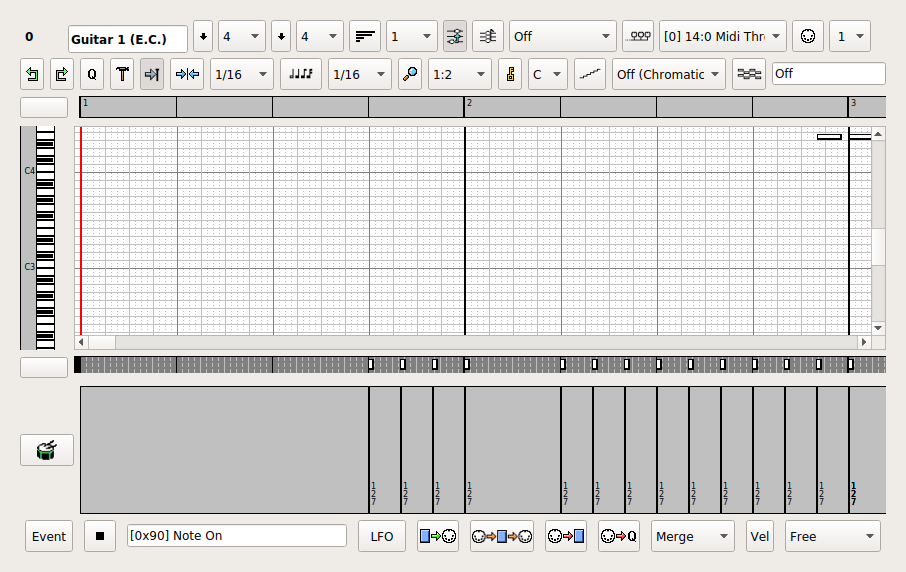
\includegraphics[scale=0.65]{roll.png}
   \caption{Stop/Pause/Start ALSA Test Setup}
   \label{fig:rc_file_stop_pause_start_alsa_test_setup}
\end{figure}

   One can copy these settings from the sample file
   \texttt{contrib/simple-midi-control-section.rc}, if one wants to
   try them.  It also illustrates some other setups that we use for testing
   purposes, but are not described here.

   Set up \textsl{VMPK} to use the lowest octave by setting
   \textbf{Base Octave} to \texttt{0}.  The red, yellow, and green
   keys shown will be our stop, pause, and start keys.
   Also set the velocity to a value ranging from 1 to 127.
   Do not use a zero velocity, as it seems that VMPK will not transmit Note On
   messages with a zero velocity.

   Next, run \textsl{Seq66}, using the following command line to make
   sure that it is using ALSA and using automatic mode to connect the ALSA MID
   ports:

   \begin{verbatim}
      $ seq66 -A -a
   \end{verbatim}
   
   Then open a MIDI file.  Next,
   open the \textbf{File / Options / MIDI Input} tab, and make sure that
   the \textbf{VMPK Output} is check-marked as shown in the figure.
   If desired, also connect up to some kind of synthesizer so that the song can
   be heard.

   Finally, press the third white key (shown as green in the figure) to start
   playback.  The second white key (yellow in the figure) will pause and resume
   playback.  The first white key (red in the figure) will stop (and rewind)
   playback.

   Then play with the BPM MIDI control keys.  Note that the size of the
   BPM step-increment and the BPM page-increment are configurable in the
   \index{usr!user-midi-settings}
   \texttt{[user-midi-settings]} section of the "usr" configuration file,
   using the following values in that section:

   \begin{verbatim}
      1        # bpm_precision
      1.0      # bpm_step_increment
      10       # bpm_page_increment
   \end{verbatim}

   See \sectionref{subsec:usr_file_user_midi_settings}; it has
   information about the usage and enabling of these settings.

   Obviously, this setup is not useful for performance, but serves as a good
   example to verify this MIDI control.

   One thing we noticed while implementing this functionality is that there
   is really no need to have two lines for pairs such as BPM up/down and
   screen-set up/down.  Also, is screen-set play now partly redundant?
   No matter, we will not break the user's existing setup.

\paragraph{Ext Automation / Performance Record}
\label{paragraph:rc_file_midi_ctrl_ex_precord}

   To do.

\paragraph{Ext Automation / Solo}
\label{paragraph:rc_file_midi_ctrl_ex_solo}

   To do.

\paragraph{Ext Automation / MIDI Thru}
\label{paragraph:rc_file_midi_ctrl_ex_thru}

   To do.

\paragraph{Ext Automation / BPM Page Up}
\label{paragraph:rc_file_midi_ctrl_ex_bpmpageup}

   To do.

\paragraph{Ext Automation / BPM Page Down}
\label{paragraph:rc_file_midi_ctrl_ex_bpmpageup}

   To do.

\paragraph{Ext Automation / Screen-Set By Number}
\label{paragraph:rc_file_midi_ctrl_ex_ssnumber}

   To do.

\paragraph{Ext Automation / MIDI Record}
\label{paragraph:rc_file_midi_ctrl_ex_mrecord}

   To do.

\paragraph{Ext Automation / MIDI Quantized Record}
\label{paragraph:rc_file_midi_ctrl_ex_qrecord}

   To do.

\paragraph{Ext Automation / Fast Forward}
\label{paragraph:rc_file_midi_ctrl_ex_fforward}

   To do.

\paragraph{Ext Automation / Rewind}
\label{paragraph:rc_file_midi_ctrl_ex_rewind}

   To do.

\paragraph{Ext Automation / Top}
\label{paragraph:rc_file_midi_ctrl_ex_top}

   To do.

\paragraph{Ext Automation / Select Playlist}
\label{paragraph:rc_file_midi_ctrl_ex_sellist}

   To do.

\paragraph{Ext Automation / Select Song}
\label{paragraph:rc_file_midi_ctrl_ex_selsong}

   To do.

\subsection{"rc" File / Mute-Group Section}
\label{subsec:rc_file_mute_group}
     
   This section is delimited by the \texttt{[mute-group]} construct.
   It controls 32 groups of mutes in the same way as defined for
   \texttt{[midi-control]}. A group is set of sequences that can toggle their
   playing state together.  Every group contains all 32 sequences in the
   active screen set.

   \begin{verbatim}
      [mute-group]
      1024    # group mute value count
      0 [0 0 0 0 0 0 0 0] [0 0 0 0 0 0 0 0] [0 0 0 0 0 0 0 0] [0 0 0 0 0 0 0 0]
      1 [0 0 0 0 0 0 0 0] [0 0 0 0 0 0 0 0] [0 0 0 0 0 0 0 0] [0 0 0 0 0 0 0 0]
      2 [0 0 0 0 0 0 0 0] [0 0 0 0 0 0 0 0] [0 0 0 0 0 0 0 0] [0 0 0 0 0 0 0 0]
      ...      ...               ...               ...               ...
      31 [0 0 0 0 0 0 0 0] [0 0 0 0 0 0 0 0] [0 0 0 0 0 0 0 0] [0 0 0 0 0 0 0 0]
   \end{verbatim}

   The initial number, 1024 is probably the total count of 32 x 32 sequences.
   In this group are the definitions of the state of the 32 sequences
   in the playing screen set when a group is selected.
   Each set of brackets defines a group:
   
   \begin{verbatim}
      [state of the first 8 sequences] [second 8] [third 8] [fourth 8]
   \end{verbatim}

   After the list of sequences and their MIDI events, one can 
   set \textsl{Seq66} to handle MIDI events and change some more settings
   in \texttt{seq66.rc}.

   What is the different between the \textbf{mute-in group}
   section and the \textbf{mute group} section?  The former defines the MIDI
   control values that can affect the muting of a group, while the latter
   specifies the patterns that are part of a group.

\subsection{"rc" File / MIDI-Clock Section}
\label{subsec:rc_file_midi_clock}

   \index{[midi-clock]}
   The MIDI Clock fields will contain the clocking state from the last 
   time \textsl{Seq66} was run.  Turn off the clock with a 0, or on
   with a 1 (which means to send MIDI Song Position, and MIDI Continue if
   starting after tick 0), or on with positioning with a 2, which sends MIDI
   Start and then begins clocking after the position reaches a modulo of the
   \textbf{Clock Start Modulo value)}.  Luckily, the user-interface makes it
   easy to select the desire value, and has tool-tips to instruct the user.
   This section has 16 entries, one for each MIDI output buss that
   \textsl{Seq66} supports.

   This configuration item is the same as the 
   \textbf{MIDI Clock} tab described in
   \paragraphref{paragraph:menu_file_options_midi_clock}
   
   Here is the format:

   \begin{verbatim}
      [midi-clock]
      16
       0 0  #  [1] seq24 1
       1 0  #  [2] seq24 2
       2 0  #  [3] seq24 3
       3 0  #  [4] seq24 4
       4 0  #  [5] seq24 5
       5 0  #  [6] seq24 6
       6 0  #  [7] seq24 7
       7 0  #  [8] seq24 8
       8 0  #  [9] seq24 9
       9 0  # [10] seq24 10
      10 0  # [11] seq24 11
      11 0  # [12] seq24 12
      12 0  # [13] seq24 13
      13 0  # [14] seq24 14
      14 0  # [15] seq24 15
      15 0  # [16] seq24 16
   \end{verbatim}

   That sample would be written one had started up \textsl{Seq66} in
   manual-mode.  On our system, where we have Timidity running, and
   erroneously have also specified 3 MIDI busses that we do not have, in the
   \texttt{seq66.usr} file:

   \begin{verbatim}
      [midi-clock]
      5    # number of MIDI clocks/busses
      # Output buss name: [0] 14:0 2x2 A (SuperNova,Q,TX81Z,DrumStation)
      0 0  # buss number, clock status
      # Output buss name: [1] 128:0 2x2 B (WaveStation,ESI-2000,MV4,ES-1,ER-1)
      1 0  # buss number, clock status
      # Output buss name: [2] 128:1 PCR-30 (303)
      2 0  # buss number, clock status
      # Output buss name: [3] 128:2 TiMidity port 2
      3 0  # buss number, clock status
      # Output buss name: [4] 128:3 TiMidity port 3
      4 0  # buss number, clock status
   \end{verbatim}

\subsection{"rc" File / MIDI-Meta-Events Section}
\label{subsec:rc_file_midi_meta_events}

   \index{[midi-meta-events]}
   The new MIDI Meta events section is the start of additional options
   supporting meta events as normal events in \textsl{Seq66}.
   \index{tempo-track-number}

   \begin{verbatim}
      [midi-meta-events]
      10      # tempo_track_number
   \end{verbatim}

   Normally, as per the MIDI specification, the first track (track 1 in track
   numbering, or pattern 0 in \textsl{Seq66} numbering) is \textsl{the}
   official track for certain MIDI meta events, such as Set Tempo and Time
   Signature.  However, to accommodate existing tunes and their set
   arrangement, we allow the user to go into \textbf{File / Options / MIDI
   Clock} and change the tempo track to another pattern.

   Please note that the user can insert Set Tempo events into any track via the
   pattern editor or the event editor.  But, when recording tempo events, they
   will always be written to the patten having the tempo-track number.

\subsection{"rc" File / Keyboard Control Section}
\label{subsec:rc_file_keyboard_control}
        
   \index{[keyboard control]}
   The keyboard control is a dump of the keys that \textsl{Seq66}
   recognises, and each key's corresponding sequence number.
   Note that the first number corresponds to the number of sequences in
   the active screen set.

   \begin{verbatim}
      [keyboard-control]
      32     # number of keys
      # Key #  Sequence #   Key name
      44  31        # comma
      49  0         # 1
      50  4         # 2
      51  8         # 3
      52  12        # 4
      53  16        # 5
      54  20        # 6
      55  24        # 7
      56  28        # 8
      97  2         # a
      98  19        # b
      99  11        # c
      100  10       # d
      101  9        # e
      102  14       # f
      103  18       # g
      104  22       # h
      105  29       # i
      106  26       # j
      107  30       # k
      109  27       # m
      110  23       # n
      113  1        # q
      114  13       # r
      115  6        # s
      116  17       # t
      117  25       # u
      118  15       # v
      119  5        # w
      120  7        # x
      121  21       # y
      122  3        # z
   \end{verbatim}

\subsection{"rc" File / Keyboard Group Section}
\label{subsec:rc_file_keyboard_group}

   \index{[keyboard-group]}
   This section is the same as
   \textbf{[keyboard-control]}, but to control groups of patterns, rather than
   individual patterns, using keystrokes.
   The keyboard group specifies more automation for the application.  The
   first number specifies the key number, and the second number specifies
   the Group number.

   Additional control items:

   \begin{enumber}
      \item \textbf{\# bpm up and down}.
         Keys to control BPM (beats per minute).
      \item \textbf{\# screen set up and down}.
         Keys for changing the active screenset.
      \item \textbf{\# group functionality on, off, learn}.
         \index{group learn}
         Note that the group learn key is a modifier key to be held while 
         \index{group toggle}
         pressing a group toggle key.
      \item \textbf{\#replace, queue, snapshot\_1, snapshot\_2, keep queue}.
         These are the other modifier keys explained in section 3a.
   \end{enumber}

   To see the required key codes when pressed, run \texttt{seq24} with
   the \texttt{--show-keys}.

   Some keys should not be assigned to control sequences in
   \textsl{Seq66} as they are already assigned in the
   \textsl{Seq66} menu (with \texttt{Ctrl}). 

   This configuration item is the same as the 
   \textbf{Keyboard} tab described in
   \sectionref{paragraph:menu_file_options_keyboard}.

   \begin{verbatim}
      [keyboard-group]
      # Key #, group # 
      32
      33  0         # exclam
      34  1         # quotedbl
      35  2         # numbersign
      36  3         # dollar
      37  4         # percent
      38  5         # ampersand
      40  7         # parenleft
      47  6         # slash
      59  31        # semicolon
      65  16        # A
      66  28        # B
      67  26        # C
      68  18        # D
      69  10        # E
      70  19        # F
      71  20        # G
      72  21        # H
      73  15        # I
      74  22        # J
      75  23        # K
      77  30        # M
      78  29        # N
      81  8         # Q
      82  11        # R
      83  17        # S
      84  12        # T
      85  14        # U
      86  27        # V
      87  9         # W
      88  25        # X
      89  13        # Y
      90  24        # Z
      39 59         # bpm up, down: apostrophe semicolon
      93 91 65360   # screen set up, down, play: bracketright bracketleft Home
      236 39 65379  # group on, off, learn: igrave apostrophe Insert
      # replace, queue, snapshot_1, snapshot 2, keep queue:
      65507 65508 65513 65514 92  # Control_L Control_R Alt_L Alt_R backslash
      1             # show_ui_sequence_key and pattern measures (1=true/0=false)
      32            # space start sequencer
      65307         # Escape stop sequencer
      0 #  show sequence numbers (1 = true / 0 = false);  ignored in legacy mode
   \end{verbatim}

   Note that most of these group-control keys are shifted versions of the
   keystrokes that control the individual sequences.  Also note the
   \texttt{Control\_L} and \texttt{Control\_R} notations a few lines above.
   \index{keys!no ctrl/alt please}
   Please avoid using any Control key combinations in the "rc"/Keyboard
   configuration.  Control keys are the province of the user-interface
   (\textsl{Gtk+}) and assigning them can cause surprising behavior!
   It is also wise to avoid the \texttt{Alt} key.

   \index{auto-shift}
   \index{group-learn!auto-shift}
   When in group-learn mode, the \texttt{Shift} key cannot be hit, so the
   group-learn mode automatically converts the keys to their shifted versions.
   \index{shift-lock}
   \index{group-learn!shift-lock}
   This feature known as \textsl{shift-lock} or \textsl{auto-shift}.

\subsection{"rc" File / JACK Transport}
\label{subsec:rc_file_jack_transport}

   This section holds the settings for both JACK transport and for native JACK
   MIDI mode.

   \index{[jack-transport]}
   The JACK Transport options are also command-line options, as indicated in
   the comments below.

   This configuration item is the same as the 
   \textbf{Jack Sync} tab described in
   \sectionref{paragraph:menu_file_options_jack_sync}.

   \index{--jack-transport}
   \index{--jack-master}
   \index{--jack-master-cond}
   \index{--jack-start-mode}
   \begin{verbatim}
      [jack-transport]
      # jack_transport - Enable slave sync with JACK Transport.
      0
      # jack_master - Seq66 attempts to serve as JACK Master.
      0
      # jack_master_cond - Seq66 is master if no other master exists.
      0
      # song_start_mode (applies mainly if JACK is enabled)
      # 0 = Playback in live mode. Allows muting and unmuting of loops.
      # 1 = Playback uses the song editor's data.
      1
   \end{verbatim}

   An additional item, new, specifies if native JACK MIDI input/output is to be
   used.

   \index{--jack-midi}
   \begin{verbatim}
      # jack_midi - Enable JACK MIDI, which is a separate option from
      # JACK Transport.
      1
   \end{verbatim}

   Please note that only \textsl{one} of
   jack\_transport, jack\_master, and jack\_master\_cond should be selected
   (set to 1) at a time.
   Also note that JACK transport is separately configurable from
   JACK MIDI, and each uses a different JACK client internally.

\subsection{"rc" File / MIDI Clock Mod Ticks}
\label{subsec:rc_file_midi_cmt}

   \index{[midi-clock-mod-ticks]}
   This configuration item is the same as the
   \textbf{Clock Start Modulo} option described in
   \paragraphref{paragraph:menu_file_options_midi_clock}.

   \begin{verbatim}
      [midi-clock-mod-ticks]
      64
   \end{verbatim}

\subsection{"rc" File / MIDI Meta Events}
\label{subsec:rc_file_midi_meta}

   This section defines some features of MIDI meta-event handling.  Normally,
   tempo events are supposed to occur in the first track (pattern 0).  But one
   can move this track elsewhere to accomodate one's existing body of tunes.
   If affects where tempo events are recorded.  The default value is 0, the
   maximum is 1023.  A pattern must exist at this number for it to work.

   \begin{verbatim}
      [midi-meta-events]
      0    # tempo_track_number
   \end{verbatim}

\subsection{"rc" File / MIDI Input}
\label{subsec:rc_file_midi_input}

   \index{[midi-input]}
   This configuration item is the same as the 
   \textbf{MIDI Input} tab described in
   \paragraphref{paragraph:menu_file_options_midi_input}.
   The "1" is a line count, and would equal the number of
   supported input ports.
   This "rc" entry here has two variables; the first is the record number or
   port number, and the second number indicates whether it is disabled (0),
   or enabled (1).

   \begin{verbatim}
      [midi-input]
      1   # number of MIDI busses
      # The first number is the port number, and the second number
      # indicates whether it is disabled (0), or enabled (1).
      # [0] 0:0 seq66 midi in
      0 0
      # If set to 1, this option allows the master MIDI bus to record
      # (filter) incoming MIDI data by channel, allocating each incoming
      # MIDI event to the sequence that is set to that channel.
      # This is an option adopted from the Seq32 project at GitHub.
      0   # flag to record incoming data by channel
   \end{verbatim}

   There is no user-interface item for the following value, but
   it does correspond to the \texttt{--manual-ports} command-line
   option.

\subsection{"rc" File / Manual ALSA Ports}
\label{subsec:rc_file_manual_ports}

   The name of this setting is a bit of a misnomer in a couple of ways:

   \index{ports!virtual}
   \index{ports!manual}
   \begin{enumerate}
      \item It actually refers to the usage of \textsl{virtual} MIDI ports.
         These are ports that are set up by the application so that other
         devices or applications can connect to the MIDI application.
         Where the "manual" idea comes in is that the user can manually choose
         the connections to be made.
      \item This option is not just for ALSA.  It can also be used when
         \textsl{Seq66} is running in native JACK mode, so support
         virtual JACK ports that can be connected manually (e.g. in the
         \textsl{QJackCtl} application.)
   \end{enumerate}

   \index{[manual-ports]}
   \begin{verbatim}
      [manual-ports]
      # Set to 1 to have seq66 create its own ALSA ports and not
      # connect to other clients.  Use 1 to expose all 16 MIDI ports to
      # JACK (e.g. via a2jmidid).  Use 0 to access the ALSA MIDI ports
      # already running on one's computer, or to use the autoconnect
      # feature (Seq66 connects to existing JACK ports on startup.
      1
   \end{verbatim}

   \index{--auto-ports}
   The opposite of \texttt{--manual-ports}
   is \texttt{--auto-ports}.  The auto-ports option
   forces \textsl{Seq66} to use the system's existing ALSA ports.
   This is necessary in order to play tunes through software synthesizers that
   use ALSA MIDI.

   \index{jack!manual-ports}
   Turning on the manual-ports option is necessary if one
   wants to use the legacy \textsl{Seq66} (\texttt{seq66})
   with JACK.
   It is \textsl{not} necessary if using the native JACK MIDI version,
   \texttt{seq66}.
   However, if one needs to avoid the auto-connect feature of \texttt{seq66},
   then the manual option is necessary.

   It will create ports as per the settings in the "user" configuration file's
   \texttt{user-midi-bus-definitions} and \texttt{user-midi-bus-N} sections.
   These definitions can be used by JACK for connection, and these definitions
   can be used to specifically rename the ports that exist in the system.
   However, this option is misleading if one wants to have access to the
   actual ALSA ports that exist on the system.
   The next option gets around that issue.

\subsection{"rc" File / Reveal ALSA Ports}
\label{subsec:rc_file_reveal_ports}

   Again, this option applies to both ALSA and native JACK.

   \index{[reveal-ports]}
   \begin{verbatim}
      [reveal-ports]
      # Set to 1 to have seq66 ignore any system port names
      # declared in the 'user' configuration file.  Use this option if
      # you want to be able to see the port names as detected by ALSA.
      1   # flag for reveal ALSA ports
   \end{verbatim}

   \index{jack!reveal-ports}
   Turning on the reveal-ports option is necessary if one
   wants to see the actual ALSA port names defined by the system.
   It will ignore the settings in the "user" configuration file's
   \texttt{user-midi-bus-definitions} and \texttt{user-midi-bus-N} sections.
   If this option is turned on, the definitions in the
   "user" configuration file are \textsl{not} read from that file.

\subsection{"rc" File / Interaction Method}
\label{subsec:rc_file_interaction}

   \index{[interaction-method]}
   This configuration item is the same as the 
   \textbf{Mouse} tab described in
   \paragraphref{paragraph:menu_file_options_mouse}.

   \begin{verbatim}
      [interaction-method]
      # 0 - 'seq24' (original seq24 method)
      # 1 - 'fruity' (similar to a certain fruity sequencer we like)
      0   # interaction_method
   \end{verbatim}

   \index{qt!fruity}
   Note that the "fruity" mouse support is not available in the Qt
   user-interface.

   \index{[allow-mod4-mode]}
   \index{new!mod4 edit-lock}
   There is an option to use the Mod4 (Super, or Windows) key in the
   Pattern Editor to lock the editing of a note.  When this mode is enabled,
   and Mod4 is pressed while the mouse right-button is released, the
   editing pencil icon remains, and notes can be added.  This feature is
   useful for crippled trackpads and trackpad drivers that cannot provide
   two simultaneous button presses.

   \begin{verbatim}
      # Set to 1 to allow seq24 to stay in note-adding mode when
      # the right-click is released while holding the Mod4 (Super or
      # Windows) key.
      1   # allow_mod4_mode
   \end{verbatim}

   \index{qt!mod4 edit-lock}
   Note that the "edit-lock" support is not available in the Qt
   user-interface.  It is just as easy to click in that pattern editor and
   press the 'p' key to enter "paint" (edit) mode.

   \index{[allow-snap-split]}
   \index{new!snap-split}
   This option comes from the \textsl{seq32} project.  It allows for
   pattern-splitting in the Song editor at snap points, rather than just
   at the middle of the pattern.

   \begin{verbatim}
      # Set to 1 to allow Seq66 to split performance editor
      # triggers at the closest snap position, instead of splitting the
      # trigger exactly in its middle.  Remember that the split is
      # activated by a middle click.
      0   # allow_snap_split
   \end{verbatim}

   \index{qt!snap-split}
   Not sure that this support is available in the Qt user-interface.

   \index{[allow-click-edit]}
   \index{new!click-edit}
   This option allows one to enable/disable the ability to double-click
   in a pattern slot in the main window to bring it up for editing.  This
   can interfere with a live performance where muting/unmuting come fast enough
   to be seen as a double-click.

   \begin{verbatim}
      # Set to 1 to allow a double-click on a slot to bring it up in
      # the pattern editor.  This is the default.  Set it to 0 if
      # it interferes with muting/unmuting a pattern.
      1   # allow_click_edit
   \end{verbatim}

   \index{qt!click-edit}
   Not sure that this support is available in the Qt user-interface.

\subsection{"rc" File / LASH Session}
\label{subsec:rc_file_lash_session}

   \index{[lash-session]}
   The following configuration item is the same as the
   \texttt{--lash} or \texttt{--no-lash} options described in
   \sectionref{sec:man_page}.
   If set to 0, LASH session support is disabled.
   If set to 1, LASH session support is enabled.
   However, if LASH support is not built into the application, neither option
   has any effect -- there is no LASH support.  
   To determine if LASH support is built in, run seq66 from the command
   line with the \texttt{--version} option, and see if LASH is mentioned.

   \begin{verbatim}
      [lash-session]
      # Set the following value to 0 to disable LASH session management.
      # Set the following value to 1 to enable LASH session management.
      # This value will have no effect is LASH support is not built into
      # the application.  Use the --help option to see if LASH is part of
      # the options list.
      1     # LASH session management support flag
   \end{verbatim}

\subsection{"rc" File / Auto Option Save}
\label{subsec:rc_file_auto_rc_save}

   \index{[auto-option-save]}
   This new item determines if the "rc" configuration file is saved
   upon exit of \textsl{Seq66}.  The legacy behavior is to save it,
   which can sometimes be inconvenient when one is just trying out some
   command-line options.

   \begin{verbatim}
      [auto-option-save]
      # Set the following value to 0 to disable the automatic saving of the
      # current configuration to the 'rc' file.  Set it to 1 to
      # follow legacy seq24 behavior of saving the configuration at exit.
      # Note that, if auto-save is set, many of the command-line settings,
      # such as the JACK/ALSA settings, are then saved to the configuration,
      # which can confuse one at first.  Also note that one currently needs
      # this option set to 1 to save the configuration, as there is not a
      # user-interface control for it at present.
      0     # auto-save-options-on-exit support flag
   \end{verbatim}

\subsection{"rc" File / Last Used Directory}
\label{subsec:rc_file_last_used_dir}

   The following item refers to the last directory in which one opened or
   saved a MIDI file.

   \index{[last-used-dir]}
   \begin{verbatim}
      [last-used-dir]
      /home/ahlstrom/Home/ca/mls/git/seq66/contrib/midi/
   \end{verbatim}

\subsection{"rc" File / Recent Files}
\label{subsec:rc_file_recent_files}

   The following item preserves a list of the last few MIDI files loaded.
   It is not filled when a MIDI file is loaded via a play-list.

   \index{[recent-files]}
   \begin{verbatim}
      [recent-files]
      4
      /home/ahlstrom/Home/ca/mls/git/seq66-alternate/contrib/midi/2Bars.midi
      contrib/midi/b4uacuse-seq24.midi
      contrib/midi/Bars.midi
      contrib/midi/b4uacuse-GM-format.midi
   \end{verbatim}

\subsection{"rc" File / Play-List}
\label{subsec:rc_file_playlist}

   This is a feature new with version 0.96.0 of \textsl{Seq66}.
   It provides a configured set of named play-lists in a play-list file,
   and a flag to activate it.
   
   \index{[playlist]}
   \begin{verbatim}
      [playlist]
      0     # playlist_active, 1 = active, 0 = do not use it
      # Provides the name of a play-list.  If there is none, use '""'.
      # Or set the flag above to 0.
      /home/ahlstrom/.config/seq66/sample.playlist
   \end{verbatim}

   See \sectionref{sec:playlist}.
   It describes the setup, layout, and usage of a
   \textsl{Seq66} playlist file containing one or more playlists.

%-------------------------------------------------------------------------------
% vim: ts=3 sw=3 et ft=tex
%-------------------------------------------------------------------------------
